\chapter{Prototipo sviluppato}
\label{chap:3}
Nel capitolo precedente sono state esaminate le differenze sostanziali tra un'approccio basato su Rust in combinazione con WebAssmebly e uno basato su Node.js.
In questo capitolo si presenterà il prototipo sviluppato con l'obiettivo di comprendere l'impatto di tali differenze in un'applicazione pratica.
\section{Descrizione dell'applicazione}
Il prototipo sviluppato è un applicazione dedicata all'elaborazione digitale di immagini, concepita per simulare un contesto realistico in cui le operazioni richiedono una considerevole quantità di elaborazioni da parte della CPU.
\\Dato il limitato tempo disponibile, non è stato possibile esplorare a fondo il contesto del \emph{digital image processing}. Sono state invece utilizzate librerie già pronte in entrambe i linguaggi, senza scendere troppo in profondità nella programmazione di basso livello.
\\L'architettura dell'applicazione seguirà un modello client-server per entrambe le implementazioni.
In particolare il cliente sarà responsabile di fornire i file da processare e le relative specifiche sulle modifiche da apportare.
Il servitore eseguirà le modifiche richieste e risponderà al client con il percorso della nuova immagine, la quale sarà pronta per essere scaricata.
\\Nel processo di selezione delle possibili modifiche da apportare, è stato essenziale individuare due librerie nei rispettivi linguaggi utilizzati.
Successivamente, per garantire uniformità nelle opzioni di modifica disponibili, sono state estratte le seguenti funzionalità comuni: 
\begin{itemize}
    \item ridimensionamento;
    \item rotazione di 90°;
    \item ribaltamento in orizzantale;
    \item conversione in bianco e nero;
    \item aumento/diminuzione del contrasto;
    \item aumento/diminuzione di luminosità;
\end{itemize}
Tali operazioni sono state selezionate poiché rappresentano funzionalità frequentemente utilizzate anche da utenti comuni, oltre a caratterizzarsi per la loro eterogeneità. Alcune di queste coinvolgono esclusivamente la manipolazione dei pixel, come ad esempio la rotazione e il ribaltamento, mentre altre, come la conversione in scala di grigi o la modifica del contrasto/luminosità, comportano modifiche dirette sui pixel stessi.
\newpage
\section{Setup sperimentale}
\section{Metodologia}
\newpage
\section{Implementazione in Rust e Wasm/WASI}
Per quanto riguarda l'implementazione si è deciso di partire dal prototipo sviluppato in Rust in quanto era l'elemento maggiormente innovativo e dispendioso in termini di tempo impiegato.
\\Si è resa inoltre necessaria la ricerca di un framework che consentisse la creazione di un web server per la gestione delle richieste utente.
\\La scelta è ricaduta su actix-web, un web framework potente ed estremamente veloce per Rust.
\\Il client è costituito una semplice pagina html contenente un form per il caricamento delle immagini e due riquadri che mostrano l'immagine pre e post modifiche. Tale pagina eseguirà una richiesta AJAX al server, il quale restituirà il percorso della nuova immagine elaborata per scaricarla.
\begin{figure}
    \begin{center}
            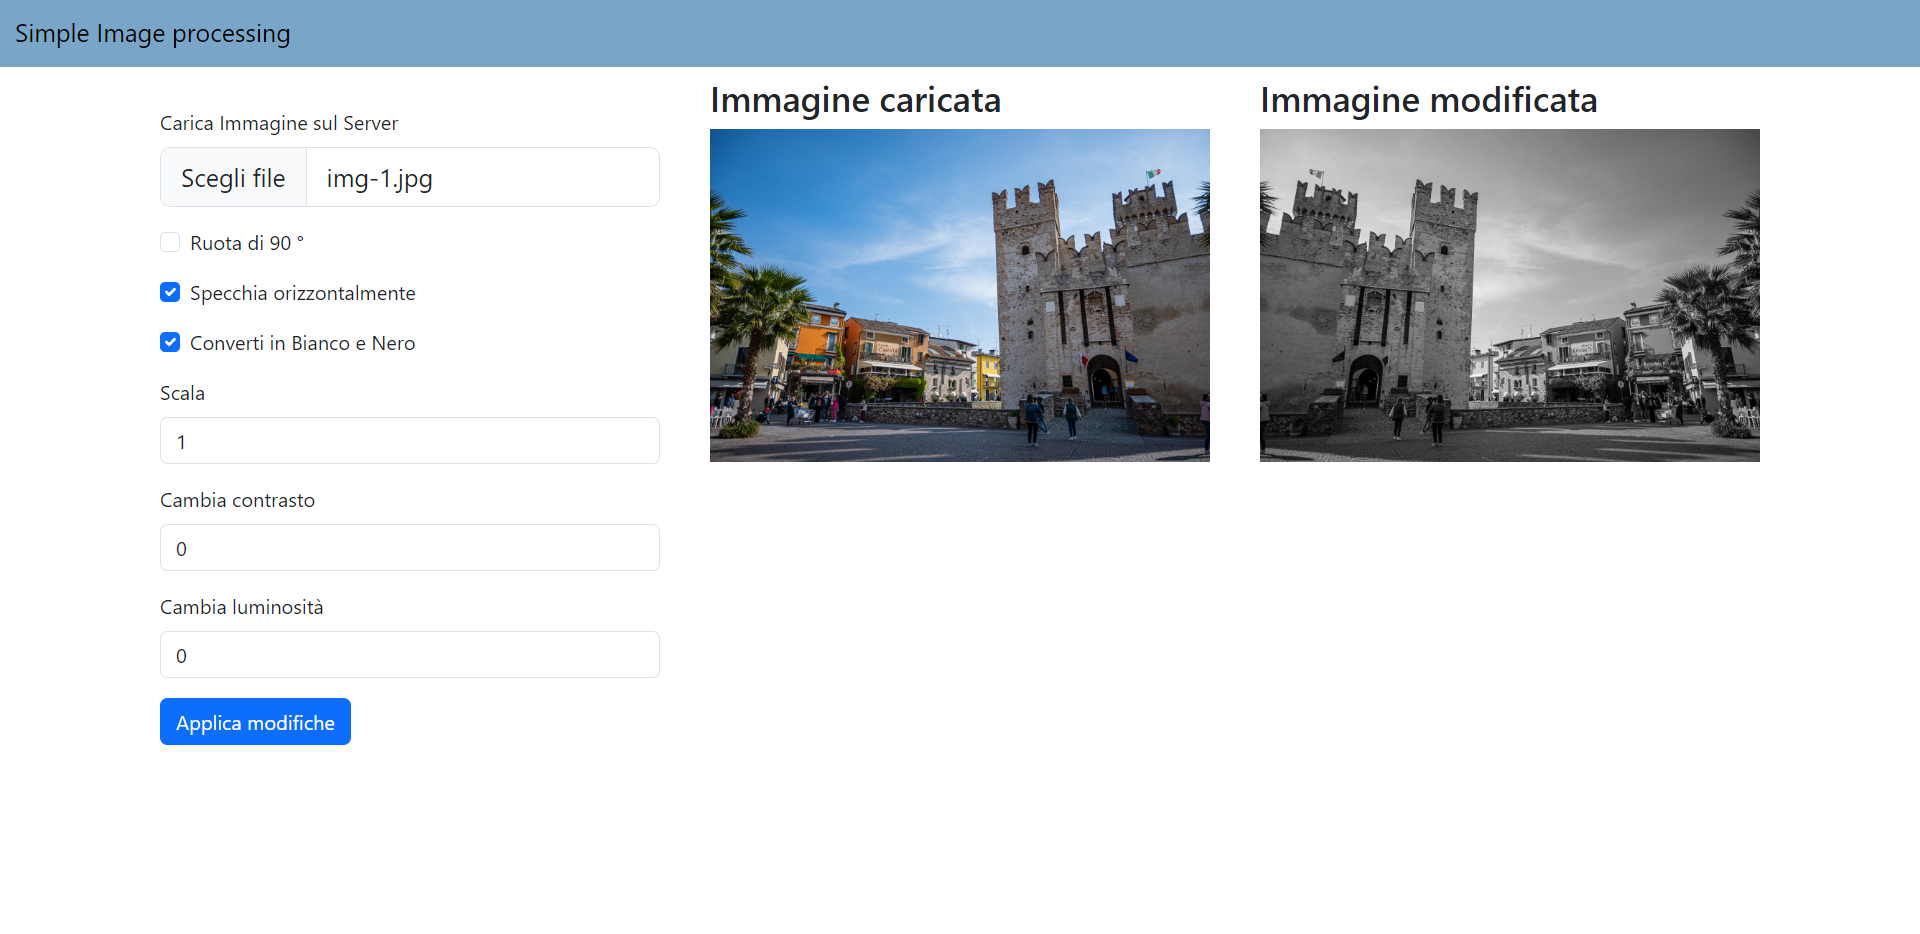
\includegraphics[width=1\columnwidth]{images/client.png}
    \end{center}
    \caption{View nel browser del client}
    \label{fig:client}
\end{figure}
\subsection{Actix-Web}
Lo studio del funzionamento di base del framework Actix-Web ha costituito un punto focale durante la prima fase dell'implementazione.
\\Tale framework si è dimostrato estremamente flessibile ed adatto per lo sviluppo di un prototipo come quello di questa tesi.
Grazie all'utilizzo di \textbf{extractors}, di \textbf{handlers} e di altre funzionalità presenti, la gestione di richieste HTTP risulta semplice ed immediata.
\\Si è deciso di strutturare l'applicazione in diversi file, garantendo così una maggior pulizia e manutenibilità del codice. Il principale tra questi è \textbf{main.rs}.
\begin{lstlisting}[language=rust, label=lst:RustWasi, caption={Porzione del file main.rs}, showstringspaces=false]
#[actix_rt::main]
async fn main() -> std::io::Result<()> {
    HttpServer::new(move || {
        App::new()
            .route("/", web::get().to(server::handlers::index))
            .route("/upload", web::post().to(server::handlers::upload))
            .service(fs::Files::new("/script", "./src/static/"))
            .service(fs::Files::new("/img", "./img/"))
            .app_data(state.clone())
    })
    .bind("127.0.0.1:8080")?
    .run()
    .await
}
\end{lstlisting}
Come si può notare è presente la creazione di un HttpServer e di un istanza di App. In Actix-web ogni server è costruiti attorno all'istanza di App.
\textbf{è presente lo state!!!!! cosa fare???} Essa permette infatti, di configurare "regole di ruoting" per risorse di vario tipo, di registrare servizi HTTP e anche di contenere stato di livello applicazione. 
\\Nel nostro caso sono state configurate due regole di routing che si riferiscono a: 
\begin{itemize}
    \item Richieste eseguite alle \textbf{home} del sito: in questo caso verrà semplicemente restituita la pagine index.html presente nella directory static;
    \item Richieste eseguite all'endpoint \textbf{\/upload}: quì sarà invece necessario ricevere un immagine e tutte le modifiche da apportare alla stessa all'interno del modulo WebAssmebly, per poi restituire il percorso della nuova immagine elaborata;
\end{itemize}
Si noti che entrambe le regole di routing mappano le richieste a funzioni presenti all'interno del file \textbf{handlers.rs} nel modulo server.
\\Successivamente sono stati registrati due servizi HTTP. Entrambi vengono utilizzati per garantire l'accesso a risorse statiche: script Javascript e immagini elaborate dall'applicazione.
\\Infine, dopo aver stabilito il metodo di dispatching delle richieste ed aver messo a disposizione le risorse necessarie ai clienti si è passati alla scrittura del codice del file \textbf{handlers.rs}. Tale file, come suggerito dal nome, contiene gli handler delle richieste HTTP, con la conseguente esecuzione di codice WebAssmebly per richieste di modifica di immagini.

\begin{lstlisting}[language=Rust,caption={Operazioni principali presenti nel file main.rs}, showstringspaces=false]
    #[derive(MultipartForm)]
    pub struct ImageUpload {
        image: TempFile,
        scala: Text<f32>,
        contrasto: Text<f32>,
        luminosita: Text<i32>,
        ruota: Text<bool>,
        specchia: Text<bool>,
        bw: Text<bool>
    }
    #[derive(Serialize, Deserialize)]
    pub struct Editings{
        scala: f32,
        ...
    }
    pub async fn index() -> HttpResponse {
        HttpResponse::Ok().content_type("text/html")
            .body(include_str!("../static/index.html"))
    }
    let new_file_name = SystemTime::now().duration_since(SystemTime::UNIX_EPOCH).unwrap();
    let filepath = format!("img/uploaded/{:?}_{}",new_file_name, form.0.file_name.as_str());
    match form.0.image.file.persist(filepath) {
            Ok(_) => {
                let editings = Editings{
                    scala : form.0.scala.0,
                    ...
                };
                edit(editings)
            },
            Err(e) => {
                HttpResponse::InternalServerError().finish()
            },
        }
    }
\end{lstlisting}
Dal listato precedente si possono facilmente notare due endpoint: il primo per richieste alla pagina home e il secondo per richieste di upload.
\\Per quanto riguarda la prima tipologia si risponde ai client semplicemente con un file HTML statico.
\\Al contrario la gestione delle richieste di upload è notevolmente più complessa e per questo motivo si è deciso di utilizzare una funzione di supporto \textbf{edit()} che si occuperà dell'istanziazione del modulo WASI e della sua esecuzione.
\\Si noti anche che la funzione "upload" riceve come parametro un MultipartForm.
Il framework Actix-Web, (ed in particolare il crate actix-multipart) facilita molto la gestione di richieste provenienti da form, anche contenenti campi di tipo "file".
Ad ognuno dei campi della struct "ImageUpload", corrisponde un parametro proveniente dalla richiesta HTML. Tali campi verranno popolati prima dell'invocazione dell'handler, rendendo possibile l'accesso immediato ai valori inviati al server.
\\Riassumendo la funzione \textbf{upload()} rende persistente il file temporaneo ricevuto ed inoltre crea un ulteriore \emph{struct} di supporto (\textbf{Editings}) che verrà sfruttata dalla funzione \textbf{edit()} per velocizzare le successive elaborazioni.
\\Si fa presente che "edit()" verrà invocata se e solo se il file è stato reso persistente senza errori, in quanto tale funzione si occuperà dell'istanziazione del modulo WebAssmebly e non avrebbe senso tentare di eseguire modifiche su un file non correttamente salvato.
\subsection{Integrazione modulo Wasm/WASI}
Come già sottolineato, per l'esecuzione di codice WebAssmebly, si è deciso di utilizzare il runtime environment \textbf{Wasmtime}. La sua integrazione all'interno di un'applicazione Rust è resa possibile primariamente grazie ai crate \textbf{wasmtime}, \textbf{wasmtime-wasi} e \textbf{wasi-common}.
\subsubsection{Scambio di dati}
Prima ancora di iniziare l'implementazione è stato necessario trovare un modo per scambiare dati tra il modulo WebAssmebly e l'host.
\\Per soddisfare i requesti imposti in questa tesi, è necessario che il modulo WebAssmebly riceva tutte le elaborazioni da effettuare su un'immagine e il nome del file da modificare, ma come introdotto in sezione \ref{subsub:Valori} una funzione WebAssmebly può accettare solamente valori di tipo numerico.
\\Grazie alle API WebAssmebly e WASI sono possibili diverse soluzioni a questo problema, come ad esempio l'utilizzo della memoria lineare, la scrittura su file, la modifica di variabili d'ambiente o la comunicazione tramite standard input.
Alcuni degli approcci presentati risulterebbero però complicati da implementare e dato che per la nostra applicazione sarebbe sufficiente scambiare una stringa per ottenere tutte le informazioni necessarie, si è optato per la comunicazione via \textbf{standard input}.
\\In particolare, per ottenere una comunicazione efficace tra host e guest, verrà implementato un protocollo composto dalla seguente sequenza di operazioni:
\begin{itemize}
    \item Serializzazione in formato JSON della struct "Editing" contenente tutte le elaborazioni  e il nome del file da modificare;
    \item Messa a disposizione sullo standard input del modulo Wasm della stringa ottenuta dalla serializzazione;
    \item Lettura della stringa dallo standard input del modulo  grazie alle API messe a disposizione da WebAssmebly System Interface;
    \item Deserializzazione in una Struct Editing equivalente a quella di partenza;
\end{itemize}
\newpage
\subsubsection{Condizioni necessarie per l'esecuzione}
Prima di poter eseguire un modulo tramite Wasmtime, sono necessarie diverse operazioni preliminari.
\\Dopo aver serializzato la struttura dati e predisposto una \textbf{ReadPipe} (crate wasi-common) per la messa a disposizione dei dati serializzati su standard input, la prima operazione necessaria è la creazione dell'\textbf{Engine} Wasmtime.
Esso rappresenta un contesto globale per la compilazione e l'esecuzione di moduli Wasm, che nel nostro specifico caso adotterà la configurazione di default.
\\Si procederà poi con l'istanziazione di un \textbf{wasmtime::Linker}. Il linker faciliterà l'istanziazione del modulo Wasm, risolvendo le diverse import (tra cui quelle per le syscall WASI).
\\Non bisogna poi dimenticare che a causa dell'architettura di WASI, sarà possibile accedere ai file presenti in una directory, se e solo se il programma avrà la capability necessarie per farlo. 
Per ottenere le capability per operare sulle immagini caricate dagli utenti, è necessario aprire la cartella "img" prima dell'istanziazione del modulo WASI.

\begin{lstlisting}[language=rust, caption={File handlers.rs: operazioni preliminari}, showstringspaces=false]
pub fn edit(editing : Editings) -> HttpResponse {
    let serialized_input = serde_json::to_string(&editing);
    let stdin = ReadPipe::from(serialized_input);
    
    let engine = Engine::default();
    
    let mut linker: Linker<WasiCtx> = Linker::new(&engine);
    wasmtime_wasi::add_to_linker(&mut linker, |s| s); 
    let  image_directory = Dir::open_ambient_dir("img", ambient_authority());
}
\end{lstlisting}
A questo punto è possibile creare e configurare un contesto WASI tramite la struct \textbf{wasmtime\_wasi::WasiCtxBuilder}.
In particolare specifichiamo che lo standard input sarà prelevato dall'oggetto contenente la serializzazione, lo standard output e lo standard error saranno ereditati dalla macchina host ed infine verrà fornita una directory precedentemente aperta, che sarà disponibile al percorso "img".
\\Sfruttando il contesto WASI è ora possibile la creazione dello \textbf{Store} Wasmtime, l'oggetto designato per l'effettiva istanziazione del modulo WebAssembly. Quest'ultimo conterrà inoltre tutte le funzioni, la memoria, le tabelle e lo stato del programma.
\begin{lstlisting}[language=rust,caption={File handlers.rs: creazione di contesto WASI e Store}, showstringspaces=false]
    let builder = WasiCtxBuilder::new()
    .stdin(Box::new(stdin.clone()))
    .inherit_stdout()
    .inherit_stderr()
    .preopened_dir(image_directory,"img");
    let wasi = builder.build();
    
    let mut store = Store::new(&engine, wasi);
\end{lstlisting}
Ora risulta inoltre possibile la creazione del \textbf{Module} WebAssmebly e il suo collegamento con il Linker, per poi finire con l'ottenimento dell'\textbf{istanza} tramite lo Store e il Module precedentemente creati.
\begin{lstlisting}[language=rust,caption={File handlers.rs: istanziazione modulo Wasm}, showstringspaces=false]
    let module = Module::from_file(&engine, "src/server/image_proc_module.wasm");
    linker.module(&mut store, "", &module) 
    let instance = linker.instantiate(&mut store, &module);
\end{lstlisting}
\subsubsection{Esecuzione del modulo WebAssmebly}
L'unica operazione rimanente è l'effettiva esecuzione della funzione del modulo WebAssmebly.
Infatti avendo configurato nel modo presentato sopra Store e contesto WASI, il programma possiede già tutti gli argomenti necessari per il corretto funzionamento.
\\Prima di poter eseguire una funzione è però necessario ottenere un'istanza di \textbf{wasmtime::Func} tramite l'operazione \emph{get\_typed\_func()} sull'istanza WebAssmebly.
A questo punto l'esecuzione è finalmente possibile grazie al metodo \emph{Func::call()}. Ad esecuzione terminata verrà eliminato lo store dalla memoria e restituito il percorso dell'immagine modificata al cliente.
\begin{lstlisting}[language=rust,caption={File handlers.rs: chiamata a funzione interna al modulo Wasm}, showstringspaces=false]
    let instance_main = instance.get_typed_func::<(), ()>(&mut store, "_start");
    instance_main.call(&mut store, ());
    drop(store);
    HttpResponse::Ok()
    .content_type("text/plain")
    .body(e.modified_file_path)
\end{lstlisting}
Si noti che in questi esempi di codice non è presente alcuna gestione degli errori. Tuttavia nel prototipo sviluppato, l'utente finale otterrà il nuovo percorso del file, se e solo se ognuna delle operazioni illustrate sarà andata a buon fine.
\subsection{Modulo WebAssmebly/WASI}
Il modulo WebAssmebly risulta a questo punto piuttosto semplice.
\\Esso si occupa infatti della lettura dei parametri da \textbf{standard input} e della loro deserializzazione in una struct Editings.
\\Successivamente vengono utilizzati i metodi forniti dal crate \textbf{image} di Rust per aprire l'immagine, modificarla secondo le specifiche ricevute dall'host e salvarla nel percorso specificato.\cite{rust:image}
\\A questo punto il controllo ritornerà all'host che si occuperà dell'invio di una risposta adeguata al client:
\begin{itemize}
    \item Se durante l'esecuzione tutte le operazioni sono terminate correttamente verrà restituito il percorso della nuova immagine generata;
    \item In caso di errore verrà restituito un errore;
\end{itemize}
\begin{lstlisting}[language=rust, showstringspaces=false]
#[derive(Serialize, Deserialize)]
pub struct Editings{
    scala: f32,
    ...
}
fn main() {
    let mut serialized_params = String::new();
    std::io::stdin().read_to_string(&mut serialized_params);
    let editings : Editings = serde_json::from_str(&serialized_params);
    let mut img = image::open(editings.filepath)
    if editings.ruota {
        img = img.rotate90();
    }
    if editings.specchia {
        img = img.fliph();
    }
    ...
    img.save(editings.modified_filepath);
}
\end{lstlisting}
Terminata la scrittura del codice, è necessario compilarlo per ottenere un modulo WebAssmebly. Ciò si può fare agovelmente grazie a \textbf{cargo}:
\begin{lstlisting}[language=Bash, numbers=none]
cargo build --release --target wasm32-wasi
        Compiling image_proc_module v0.1.0 (.\esempio_wasi)
            Finished release [optimized] target(s) in 1.21s
\end{lstlisting}
In questo particolare caso risulta molto importante la presenza del flag \textbf{- - release}, in quanto diverse funzioni del crate image, sono estremamente lente in debug mode.
\\Si noti anche che, in quanto abbiamo svolto tutte le operazioni necessarie nel main, nel momento in cui l'host invocherà il metodo \emph{get\_typed\_func()}, sarà necessario specificare la funzione chiamata \textbf{\_start}.



\newpage
\section{Implementazione in Node.js}

\section{Valutazione delle prestazioni}
\section{Qualità del codice e manutenibilità}
\section{Esperienza di sviluppo}
\section{Scalabilità e concorrenza}
\section{Conclusioni}
\section{Sviluppi futuri}



\begin{lstlisting}[language=rust, showstringspaces=false]
\end{lstlisting}